\section{Transformation und Koordinatensysteme}
	\subsection{Motivation}
	\textbf{Problem}:	Bisher ist war es uns nur möglich über Quader oder Normalbereiche zu integrieren. Es fehlt eine universelle Möglichkeit. \newline
	\textbf{Idee}: 1-dimensionale Substitution $\int_{x(a)}^{x(b)} f(t) \;dt = \int_a^b f(x(u))x'(u)\;du$.
	$\Rightarrow$ Es wird ein Integral über dem Intervall $(x(a), x(b))$ durch ein Integral über dem Intervall $(a,b)$ angenähert. \newline
	Ist es möglich ein Gebietsintegral über einem komplizierten Gebiet $D$ durch ein Integral über einem einfachen Gebiet $B$ darzustellen?\newline
	\textbf{Also}:
	\begin{equation}
		\int_D f(\vec{x})\;d\vec{x} = \int_B g(\vec{y})\;d\vec{y}
	\end{equation}
	Wobei $B$ idealerweise ein Normalbereich sein sollte. Wir brauchen eine Verknüpfung beider Integrale!
	\begin{equation*}
		\Rightarrow \Psi: B \to D
	\end{equation*}
	\textbf{Idee}: 1-dimensionale Substitutionsregel nutzt die Ableitung der Funktion. Funktioniert das analog im n-dimensionalen mit der Jacobi-Matrix?
	
	 \subsection{Transformation}
	 Eine Transformation bewirkt einen Wechsel des Koordinatensystems. Wir stellen folgende Bedingungen an die Transformationsabbildung:
	 \begin{description}
	 	\item[(1) ] Sie soll bijektiv sein. \\
	 	\item[(2) ] Sie soll stetig differenzierbar sein und für die Funktionaldeterminanten soll
	 	\begin{equation}
	 		\det \Psi'(\vec{x}) < 0 \text{ oder } \det \Psi'(\vec{x}) > 0
	 	\end{equation}
	 	f.f.a. $\vec{x} \in B$ gelten.
	 	\textbf{(1)} Stellt dabei sicher, dass das komplette Volumen von $B$ berücksichtigt wird und das keine Bereiche doppelt gezählt werden. \textbf{(2)} vermeidet Widersprüche durch konstruierte Funktionen die z.B. bei einer Transformation zu einer Nullmenge führen würden.
	 \end{description}
	 
	 \begin{bem}
	 	Die Funktionaldeterminante ist gegeben durch
	 	\begin{equation}
	 		\Psi' := |J(f(\vec{x}))|
	 	\end{equation}
	 \end{bem}
	 
	 Für $B,D$ und $\Psi: B \to D$ sollen die eben formulierten Vorraussetzungen gelten. Eine Funktion $f: D\to \R$ ist genau dann über $D$ integrierbar, wenn $f(\Psi(\cdot))|det \Psi'|$ über $B$ integrierbar ist und es gilt
	 \begin{equation}
	 	\int_D f(\vec{x}) \; d\vec{x} = \int_B f(\Psi(\vec{y})) |det \Psi'(\vec{y})| \; d\vec{y} = \int_B f(\vec{u}) |det J_{\vec{x}}(\vec{u})| \; dB
	 \end{equation}
	 
	 \subsubsection{Ablauf der Koordinatentransformation}\label{subs:abl_koordinatentrans}
	 Der allgemeine Ablauf einer Koordinatentransformation soll hier anhand einer Oberflächeninteration gezeigt werden.
	\begin{flalign*}
    	&\text{Angaben zum Beispiel}&
  	\end{flalign*}
  	Zu bestimmen ist der Flächeninhalt des folgenden Graphen:
  	\begin{equation}
  		f_1:\lbrace(x,y) \in \R^2| 1 \leq x^2 + y^2 \leq 4 \rbrace \to \R,\quad (x,y) \mapsto xy
  	\end{equation}
  	\begin{figure}[H] 
		  \centering
		  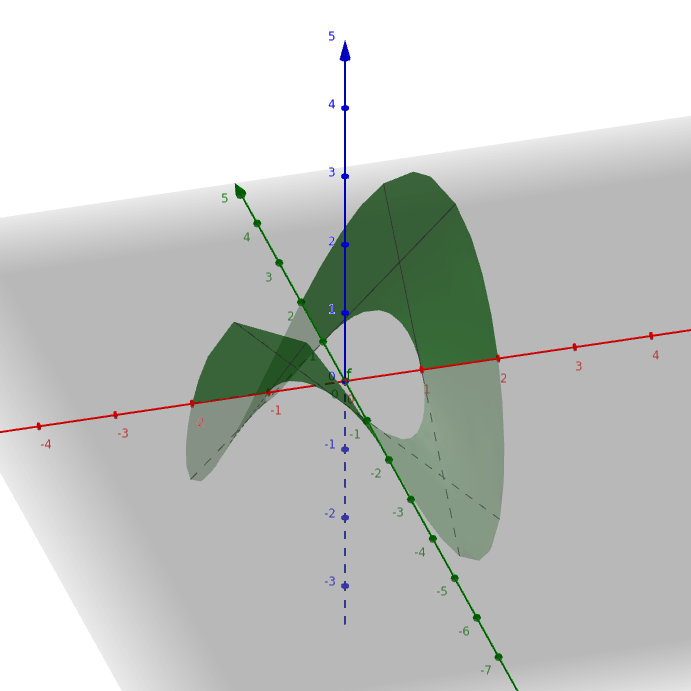
\includegraphics[width=0.5\textwidth]{./img/transf_bsp_a.png}
		  \caption{Zu untersuchendes Gebiet}
		  \label{fig:transf_bsp_a}
	  \end{figure}
	  \vspace{-1cm}
	\begin{flalign*}
    &\textbf{Schritt 1: } \text{Vektorfeld aus den Angaben schließen}&
  \end{flalign*}
    \vspace{-0.5cm}
    \begin{align}
    	v\vec{v} = \vecT{x \\ y \\xy}
    \end{align}
      \vspace{-0.5cm}
  \begin{flalign*}
    &\textbf{Schritt 2: } \text{Allgemeines Oberflächenintegral aufstellen und vereinfachen}&
  \end{flalign*}
    \vspace{-0.5cm}
  \begin{align*}
    O_F(f_1)  &= \int_F \;d\sigma = \int_B \left| \left| \frac{\partial \vec{v}}{\partial x} \times \frac{\partial \vec{v}}{\partial y} \right| \right| \; d(x,y) \\
    &= \int_B \sqrt{y^2 + x^2 + 1} \;d(x,y)
  \end{align*}
    \vspace{-0.5cm}
  \begin{flalign*}
    &\textbf{Schritt 3: } \text{Parametrisierung auf die transformiert werden soll aufstellen (hier Polarkoordinaten)}&
  \end{flalign*}
    \vspace{-0.5cm}
  \begin{align*}
  	\gamma = \vecT{r \cdot \cos \varphi \\ r \cdot \sin \varphi} \quad, 1 \leq r \leq 2,\; 0 \leq \varphi \leq 2\pi
  \end{align*}
  Wobei zu beachten ist, dass $\gamma_1$ analog zu $\gamma$ parametrisiert ist. Einzig geändert hat sich die obere Schranke für $r$ wie unschwer an den Integralsgrenzen zu erkennen ist.
  \begin{flalign*}
    &\textbf{Schritt 4: } \text{Verzerrungsfaktor berechnen}&
  \end{flalign*}	
	 \vspace{-0.5cm}
  \begin{align*}
  	\left| \det J_{\gamma}(r,\varphi)\right| = \left| 
  	\begin{array}{c c}
  		\cos \varphi & -r \sin \varphi \\
  		\sin \varphi & r \cos \varphi
	\end{array}  	  \right| = r
  \end{align*}
  \vspace{-0.5cm}
	 \begin{flalign*}
    &\textbf{Schritt 5: } \text{Transformationsparametrisierung und Verzerrungsfaktor einsetzen}&
  \end{flalign*}	
	 \vspace{-0.5cm}
  \begin{align*}
  O_F(f_1) &= \int_0^{2\pi} \int_1^2 \sqrt{r^2 + 1} r \; dr d\varphi \quad, \text{ mit }u:= 1+r^2 \Rightarrow du= 2r \;dr \text{ folgt} \\
  &= \frac{1}{2} \int_0^{2\pi} \int_{1+1^2}^{1+2^2} \sqrt{u} \;du d\varphi = \frac{1}{2} \int_0^{2\pi} \frac{2}{3} u^{\frac{3}{2}}\Big|_2^5 \; d\varphi = \pi \frac{2}{3} \left(\sqrt{5^3} - \sqrt{2^3}\right) = \frac{2\pi}{3} \left(5 \sqrt{5} - 2\sqrt{2}\right)
  \end{align*}  
	 
	 \subsection{Wichtige Koordinatensysteme}
	 \subsubsection{Polarkoordinaten}
	 Im $\R^2$ gegeben durch eine Parametrisierung mit $(r,\varphi)$, wobei $0 \leq r$ den Abstand eines Punktes vom Ursprung und $\varphi \in (-\pi, \pi)$ den Winkel zwischen der Verbindungsstrecke des Punktes mit dem Ursprung und der positiven $x-1$-Achse bezeichnet. Die Parametrisierung ist gegeben durch;
	 \begin{align}
	 	\Psi(r,\varphi) = \vecT{  r\cdot \cos \varphi \\ r \cdot \sin \varphi} \qquad, (r,\varphi) \in B \\
	 	\text{mit } 0\leq \text{ und } -\pi \leq \varphi \leq \pi \text{ oder } 0 \leq \varphi \leq 2\pi \nonumber 
	 \end{align}
	 damit ergibt sich
	 \begin{align}
	 J_{\Psi}(r, \varphi) &= \left(
	 	\begin{array}{c c}
	 		\cos \varphi & -r \sin \varphi \\
	 		\sin \varphi & r \cos \varphi
	 	\end{array}  \right) \\
	 	\Rightarrow \Psi'(r,\varphi) &= r \cos^2 \varphi + r \sin^2 \varphi = r
	 \end{align}
	 Ist $D \subset \R^2$, $f \in L(D)$ und $B$ die Beschreibung von $D$ durch Polarkoordinaten, so gilt
	 \begin{equation}
	 	\int_D f(x_1,x_2) \; d(x_1,x_2) = \int_B f(r \cos \varphi, r \sin \varphi) r \; d(r,\varphi)
	 \end{equation}
	 
	 \subsubsection{Zylinderkoordinaten}
	 Zylinderkoordinaten erweitern Polarkoordinaten um eine dritte Dimension. Es wird praktisch einfach eine dritte Koordinate angefügt. Damit ergibt sich für die Parametrisierung
	 \begin{align}
	 	\Psi(r,\varphi,z) &= \vecT{r\cdot \cos \varphi \\ r \cdot \sin \varphi \\ z} \\
	 	\text{mit } (r,\varphi,z) \in B \text{, } 0\leq r &\text{ und } -\pi \leq \varphi \leq pi \text{ oder } 0 \leq \varphi \leq 2\pi \nonumber
	 \end{align}
	 Damit ergibt sich 
	 \begin{align}
	 	J_{\Psi} (r,\varphi,z) &= \left(
	 	\begin{array}{c c c}
	 		\cos \varphi & -r \sin \varphi & 0 \\
	 		\sin \varphi & r \cos \varphi & 0 \\
	 		0 & 0 & 1	 	
	 	\end{array} \right) \\
	 	&\Rightarrow \Psi'(r,\varphi,z) = r
	 \end{align}
	 Ist $D \subset \R^3$, $f \in L(D)$ und $B$ die Beschreibung von $D$ durch Zylinderkoordinaten, so gilt
	 \begin{equation}
	 	\int_D f(x_1,x_2,x_3) \; d(x_1,x_2,x_3) = \int_B f(r \cos \varphi, r \sin \varphi,z) r \; d(r,\varphi,z)
	 \end{equation}
	 
	 \subsubsection{Kugelkoordinaten}
	 Man überträgt die Idee der Darstellung durch einen Abstand $r$ und Winkel $\varphi$ wie aus den Polarkoordinaten bekannt auf den $\R^3$. Zusätzlich variiert man einen Winkel um die $z$-Koordinate herum. So ergibt sich die Parametrisierung zu:
	 \begin{align}
	 	\Psi (r,\varphi,\vartheta) = \vecT{r \cos \varphi \sin \vartheta \\ r \sin \varphi \sin \vartheta \\ r \cos \vartheta} \\
	 	\text{mit } 0 \leq r ,\; -\pi \leq \varphi \leq \pi, \; 0 \leq \vartheta \leq \pi \nonumber
	 \end{align}
	 Damit ergibt sich
	 \begin{align}
	 	J_{\Psi}(r, \varphi, \vartheta) &= \left(
	 	\begin{array}{c c c}
	 		\cos \varphi \sin \vartheta & -r \sin \varphi \sin \vartheta & r \cos \varphi \cos \vartheta \\
	 		sin \varphi \sin \vartheta & r \cos \varphi \cos \vartheta & r \sin \varphi \cos \vartheta \\
	 		\cos \vartheta & 0 & -r \sin \vartheta
	 	\end{array} \right) \\
	 	&\Rightarrow \Psi'(r,\varphi, \vartheta) = -r^2 \sin \vartheta
	 \end{align}
	 Ist $D \subset \R^3$, $f \in L(D)$ und $B$ die Beschreibung von $D$ durch Kugelkoordinaten, so gilt
	 \begin{align}
	 	\int_D f(x_1,x_2,x_3) \;&d(x1,x2,x3) \nonumber \\
	 	&= \int_b f(r \cos \varphi \sin \vartheta, r \sin \varphi \sin \vartheta, r \cos \vartheta) \cdot r^2 \sin \vartheta \;d(r,\varphi, \vartheta)
	 \end{align}
	